\documentclass{standalone}
\usepackage{tikz}
\usepackage{verbatim}
\usetikzlibrary{positioning}
\begin{document}
\pagestyle{empty}
  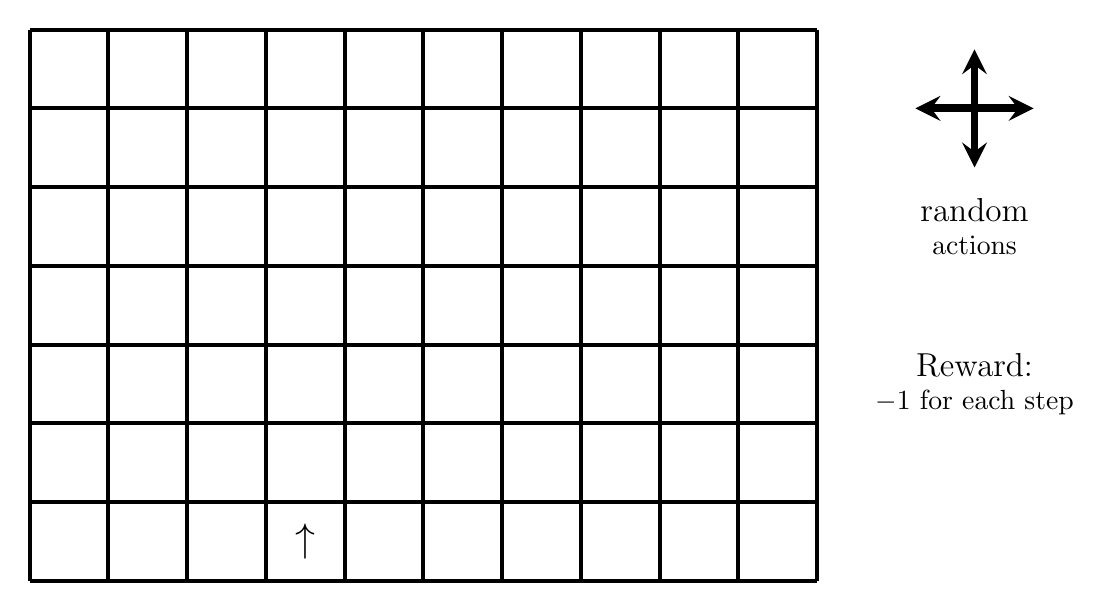
\begin{tikzpicture}
    \draw[stealth-stealth, line width=1 mm] (12.75, 6) -- (11.25, 6);
    \draw[stealth-stealth, line width=1 mm] (12, 5.25) -- (12, 6.75);
    \node[align=center] at (12, 4.5) {\large random\\actions};
    \node[align=center] at (12, 2.5) {\large Reward: \\$-1$ for each step};
    for
    \node at (3.5, 0.5) {\Large $\uparrow$};


    \draw[step=1.0,black, line width=0.5 mm] (0,0) grid (10, 7);
  \end{tikzpicture}
\end{document}